\chapter{Complementary information}
\label{app:complement}

\section{Jury Sunshine Irregularities} \label{app:irregs}

\begin{table}[h]
  \caption[Jury Sunshine Irregularities]{Jury sunshine data irregularities noted in data flattening}
  \centering
  \begin{tabularx}{\textwidth}{|c|X|} \hline
    Charges without trial (ACISID) & 08CRS50940, 08CRS52888, 09CRS000305, 09CRS1106, 09CRS50752, 10CR52031, 10CRS051975,
    10CRS1215, 10CRS397, 10CRS51388, 10CRS51610, 10CRS52410, 11CRS051642, 11CRS051795, 11CRS1577, 11CRS1745, 11CRS1783,
    11CRS51204, 11CRS51895, 11CRS52470, 08CRS54836, 08CRS50113 \\ \hline 
    Prosecutors without trials (IDs) & 1-000, 11B-000, 12-000, 14-000, 15B-000, 16A-000,
                     16B-000, 17A-000, 17B-000, 19A-000, 19B-000,
                     20A-000, 20B-000, 21-000, 22A-000, 22B-000,
                     24-000, 25-000, 27A-000, 27B-000, 28-000,
                                       29A-000, 29B-000, 30-000, 6-000, 9-000 \\ \hline
    Trial missing charge (ID) & 710-01 \\ \hline
  \end{tabularx}
\end{table}

\section{Jury Sunshine Charge Classification} \label{app:charge}

\begin{figure}[!h]
  \centering
  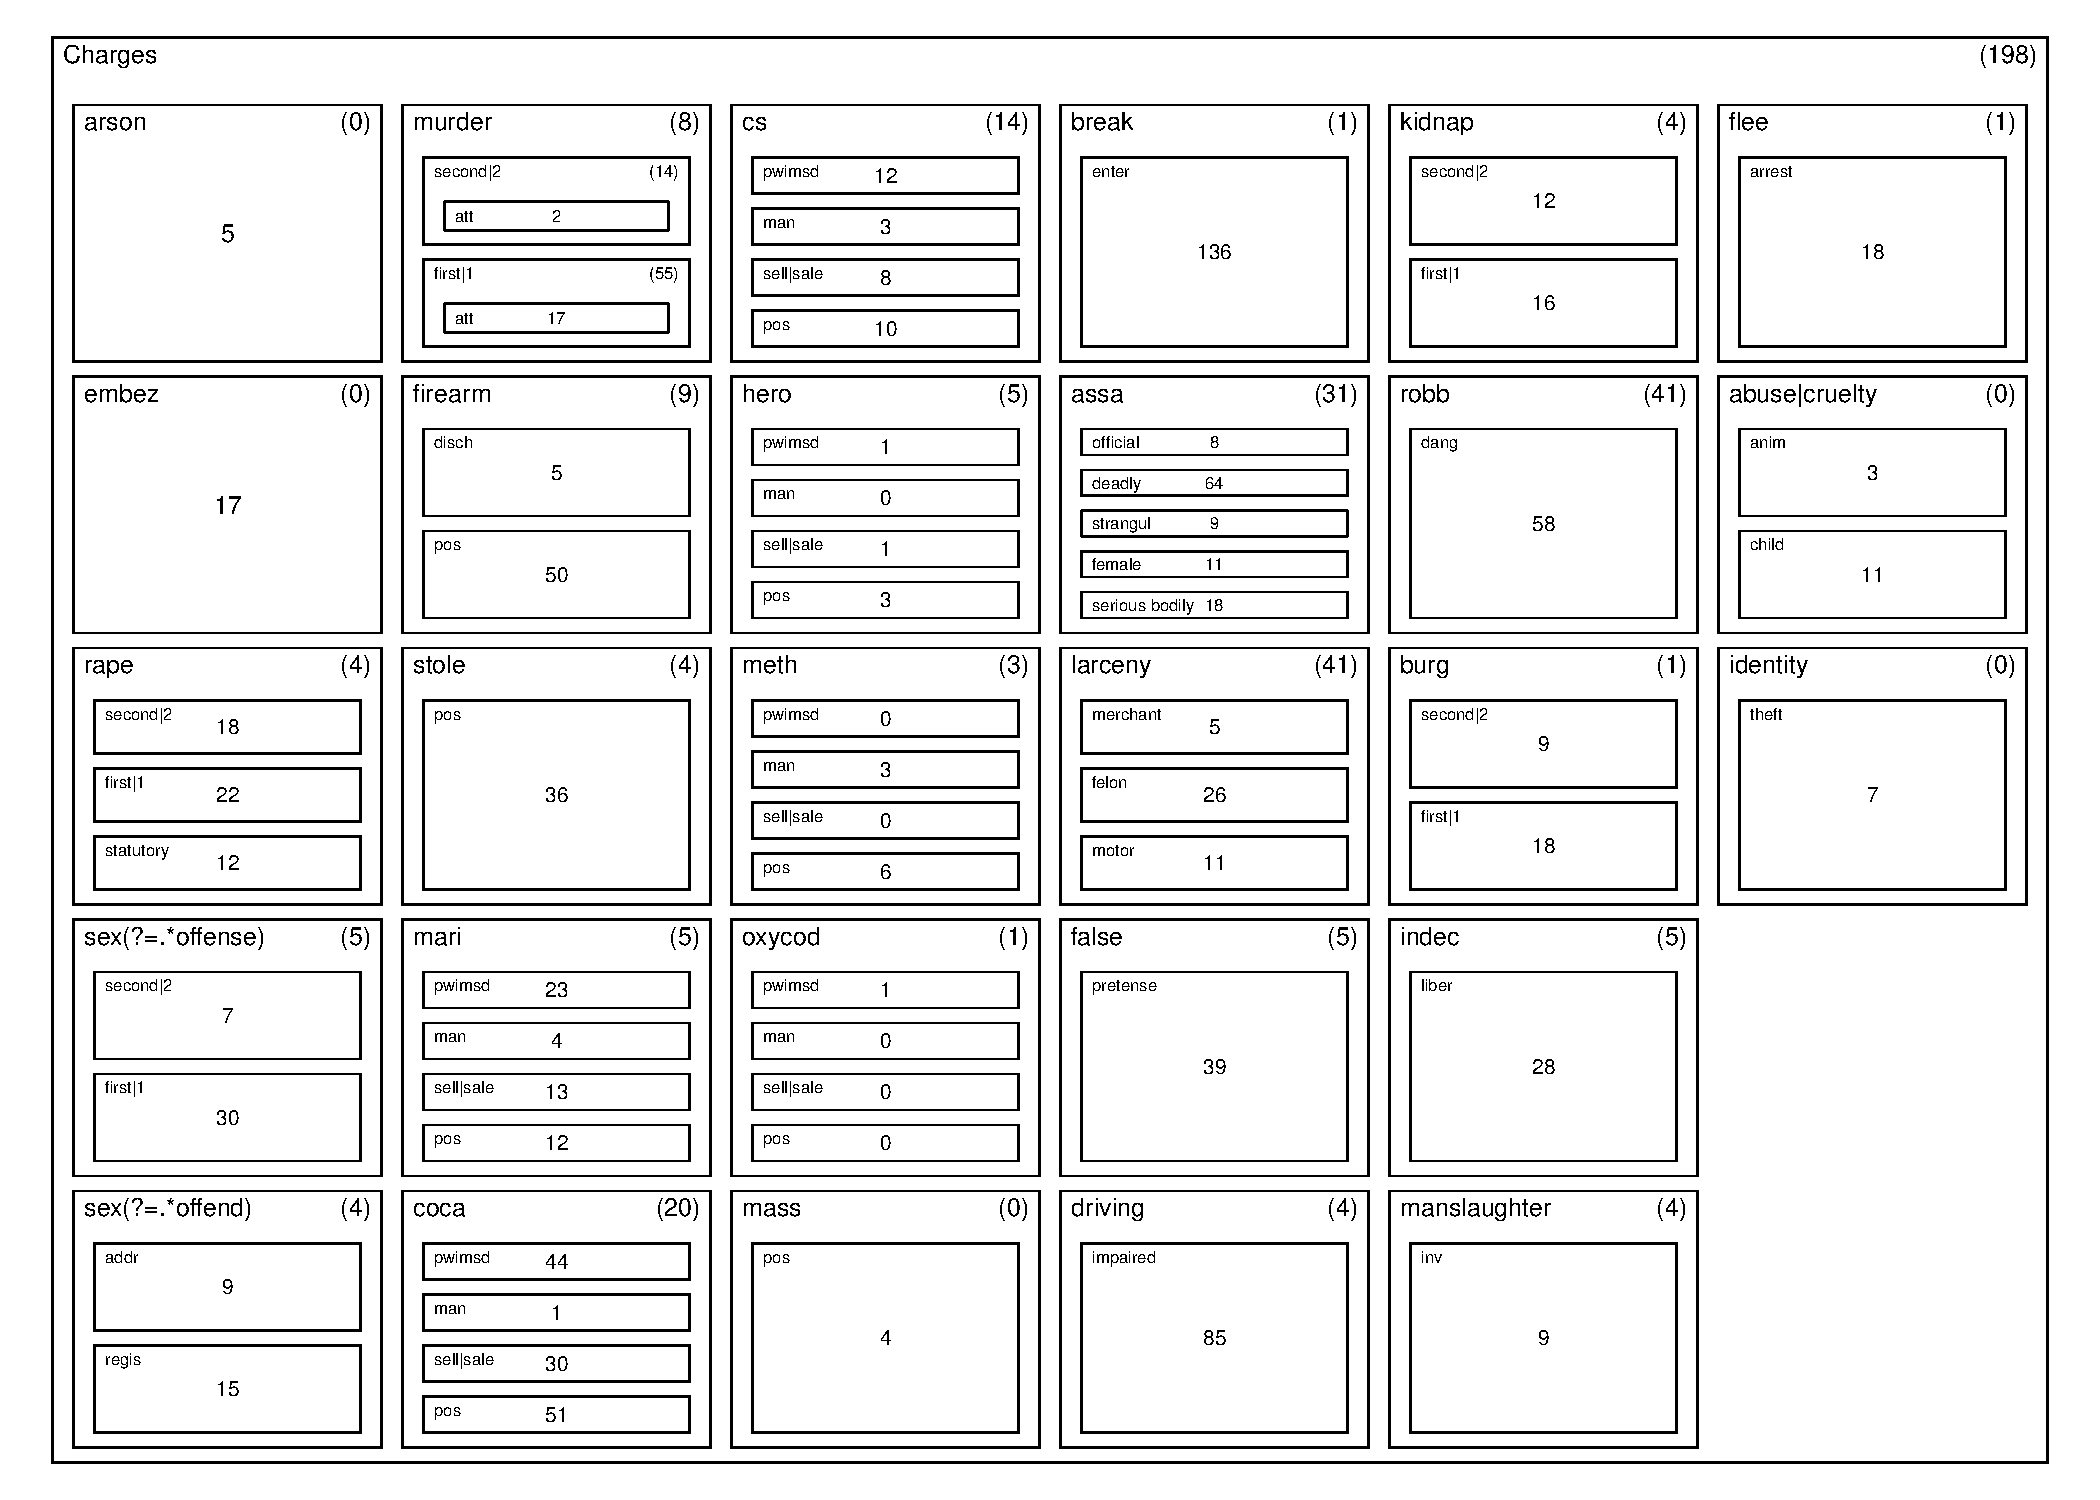
\includegraphics[angle=90, origin=c, width=1\textwidth]{ChargeDiagram}
  \caption[Regular expression charge tree visualized]{The regular expression charge tree arranged by hierarchy with counts
    provided. The counts in brackets indicate the counts of charges which could not be classified to a lower level of the
    hierarchy}
  \label{fig:chargetree}
\end{figure}

%%% Local Variables: 
%%% mode: latex
%%% TeX-master: "MasterThesisSfS"
%%% End: 
